%\documentclass[aspectratio=169, handout]{beamer}
\documentclass[aspectratio=169]{beamer}


\makeatletter
\renewcommand*\env@matrix[1][\arraystretch]{%
  \edef\arraystretch{#1}%
  \hskip -\arraycolsep
  \let\@ifnextchar\new@ifnextchar
  \array{*\c@MaxMatrixCols c}}
\makeatother

\usepackage{tikz}
\usetikzlibrary{tikzmark,fit,shapes.geometric}


\newcommand{\transp}{^{\rm{T}}}

\usepackage{cases}
\usepackage[english]{babel}
% or whatever
\usepackage{xcolor}
\usepackage{colortbl}
\usepackage[latin1]{inputenc}
\usepackage[super]{nth}
% or whatever
%\setbeamertemplate{footline}[page number]
\setbeamertemplate{footline}
        {
      \leavevmode%
      \hbox{%
      \begin{beamercolorbox}[wd=.333333\paperwidth,ht=2.25ex,dp=1ex,center]{author in head/foot}%
        \usebeamerfont{author in head/foot}\insertshortauthor%~~(\insertshortinstitute)
      \end{beamercolorbox}%
      \begin{beamercolorbox}[wd=.333333\paperwidth,ht=2.25ex,dp=1ex,center]{title in head/foot}%
        \usebeamerfont{title in head/foot}\insertshorttitle
      \end{beamercolorbox}%
      \begin{beamercolorbox}[wd=.333333\paperwidth,ht=2.25ex,dp=1ex,right]{date in head/foot}%
        \usebeamerfont{date in head/foot}\insertshortdate{}\hspace*{2em} \insertframenumber{}  \hspace*{2em}%/ \inserttotalframenumber\hspace*{2ex} 

    %#turning the next line into a comment, erases the frame numbers
        

      \end{beamercolorbox}}%
      \vskip 0pt%
    }

\usepackage{times}
\usepackage[T1]{fontenc}
\usepackage{psfrag}
\usepackage{algorithm}
\usepackage{amsmath}
\usepackage{amssymb}
\usepackage{tabularx}
\usepackage{algpseudocode}
\usepackage{mathrsfs}
\usepackage{textpos}
\usepackage{graphicx}
\usepackage{tcolorbox}
\usepackage{multicol}
\usepackage{tikz}
\usetikzlibrary{arrows.meta,shapes.arrows}
%\setkeys{Gin}{draft}
\usepackage{caption}
\captionsetup{font=scriptsize,labelfont=scriptsize}
\usepackage{color}
\DeclareCaptionFont{blue}{\color{blue}}
\captionsetup{labelfont=blue}
\usepackage{tikz}
\tikzset{
  every overlay node/.style={
    draw=white,anchor=north west,
  },
}
\def\checkmark{\tikz\fill[scale=0.4](0,.35) -- (.25,0) -- (1,.7) -- (.25,.15) -- cycle;}
\def\tikzoverlay{%
   \tikz[baseline,overlay]\node[every overlay node]
}%
%\DeclareGraphicsRule{.png}{png}{.png.bb}{}

\newtheorem{assumption}{Assumption} %jw

\newcommand{\T}{{\rm T}}

\newcommand\blfootnote[1]{%
  \begingroup
  \renewcommand\thefootnote{}\footnote{#1}%
  \addtocounter{footnote}{-1}%
  \endgroup
}
\setcounter{tocdepth}{1}
\beamertemplatenavigationsymbolsempty


\title[Lecture 11: Regression wrapup] % (optional, use only with long paper titles)
{Data, Environment and Society: \\{Lecture 11: Linear Regression Wrapup}}


%\subtitle
%{Include Only If Paper Has a Subtitle}

\author[ER131: Data, Environment and Society] 
{Instructor: Duncan Callaway\\
GSI: Salma Elmallah} 
% - Give the names in the same order as the appear in the paper.
% - Use the \inst{?} command only if the authors have different
%   affiliation.

%\logo{
%\includegraphics[width=1.5cm,height=1.5cm,keepaspectratio]{uvic_logo_h.jpg}
%}
\vspace{-20mm}
\institute[UC Berkeley] % (optional, but mostly needed)
 {\small{ \bf October 3, 2019}}


\date[October 3, 2019]


\begin{document}

\begin{frame}[plain, noframenumbering]
  \titlepage
\end{frame}

\begin{frame}{Announcements}

\textbf{Today}
\begin{itemize}
\item Quantitative vs qualitative (categorical) features
\item Nonlinear features
\item A few things to watch out for in OLS
\end{itemize}

\textbf{Reading}
\begin{itemize}
\item Tuesday: DS100 Ch 11 (Gradient descent) and Novotny \textit{et al}
\item Next Thursday: ISLR 5.1-5.2 (Resampling)
\end{itemize}
\end{frame}


\begin{frame}{Prediction models in the news}

\begin{columns}
\column{0.5\textwidth}
\begin{figure}
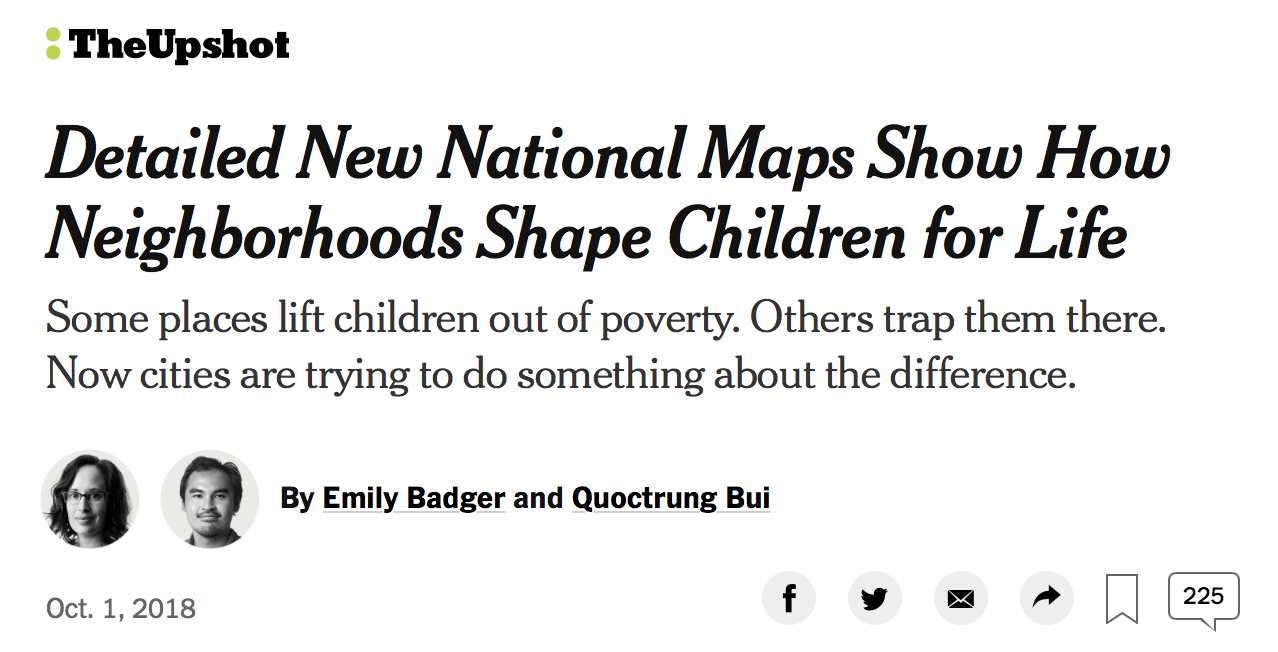
\includegraphics[width=\textwidth]{NYT_poverty_maps}
\caption*{}
\end{figure}
\column{0.5\textwidth}
``The Opportunity Atlas is built using anonymized data on 20 million Americans who are in their mid-thirties today. We map these individuals back to the Census tract (geographic units consisting of about 4,200 people) in which they grew up. Then, for each of the 70,000 tracts in America, we estimate children's average earnings, incarceration rates, and other outcomes by their parental income level, race, and gender.''
\end{columns}
\end{frame}

\begin{frame}{Prediction in the news, continued}

\begin{columns}
\column{0.7\textwidth}
\begin{figure}
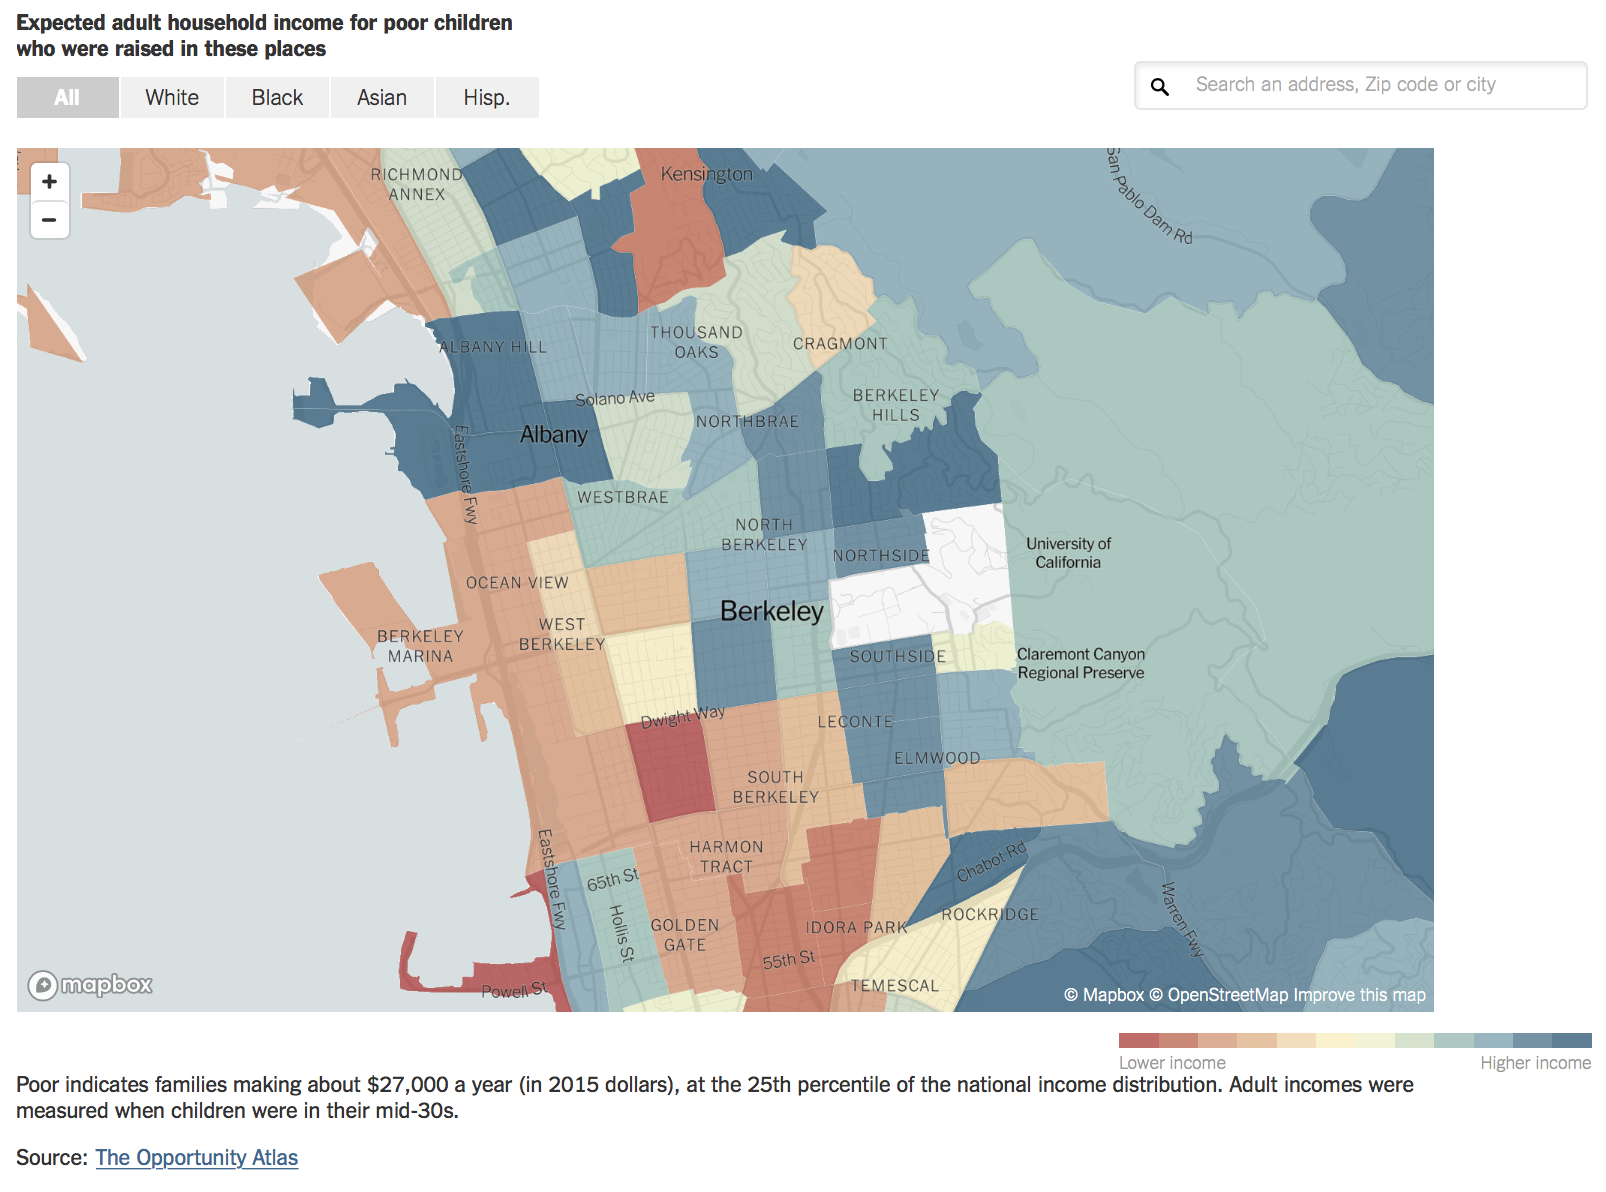
\includegraphics[height=0.8\textheight]{opportunityatlas}
\caption*{}
\end{figure}
\column{0.3\textwidth}
\href{https://www.nytimes.com/2018/10/01/upshot/maps-neighborhoods-shape-child-poverty.html}{More exploring \textbf{here}}
\end{columns}
\end{frame}

\begin{frame}{If you were a policy-maker...}
How would you use the information in these maps?

\begin{itemize}
  \item Head Start centers
  \item Tax benefits
  \item Priority for selective schools (not race-based?)
  \item Allocate resources to the places with the most upward mobility?
  \item Allocate resources to the places with the lowest income potential?
\end{itemize}

What would you question about the validity of the predictions?
\begin{itemize}
  \item These are for kids raised 30+ years ago -- are things still the same?
\end{itemize}
\end{frame}

\begin{frame}{Is this a qualitative predictor?}

Pop-up shops are a marketing gimmick to get Duncan to think shopping is fun.

\begin{enumerate}
\item Strongly disagree
\item Disagree
\item Neither agree nor disagree
\item Agree
\item Strongly agree
\end{enumerate}

\vspace{5mm}

\textbf{Answer}: \pause  This is not a qualitative variable: it categorizes someone's opinion on a numeric scale.  The responses can be \textit{ordered} from one extreme to another.  (The scale is called the \textit{Likert scale}.)

\end{frame}

\begin{frame}{Qualitative or not?}

What is your favorite type of soup?
\begin{enumerate}
\item Split pea
\item Minestrone
\item Other
\item I don't like soup
\end{enumerate}

\vspace{5mm}

\textbf{Answer}: \pause This is a qualitative predictor.  There is no context in which these answers can be sorted or summed together.

\end{frame}

\begin{frame}{Qualitative or not?}

\begin{enumerate}
\item Red
\item Orange
\item Yellow
\item Green
\item Blue
\item Indigo
\item Violet
\end{enumerate}

\vspace{5mm}

\textbf{Answer}: \pause This could be a qualitative variable \textit{or } a quantitative one.  Quantitative might make sense if we're doing research that relates to color frequency spectra (these are ordered in the sequence of the rainbow).  Qualitative might make sense if we're trying to understand what color clothing people like to buy.

\end{frame}

\begin{frame}{Qualitative predictor?}

What type of roofing material?
\begin{enumerate}
\item Thatched
\item Corrugated Metal
\item Composition shingle
\item Clay tile
\end{enumerate}

\vspace{5mm}

\textbf{Answer}: \pause Again, depends on context.  Often roof material is used as a measure of wealth for household surveys in low income countries.  But one might also be asking for people's aesthetic preferences, in which case the connection to wealth may not be relevant.  

\end{frame}

\begin{frame}{Qualitative predictors, defined}

\textbf{Quant}itative predictors 
\begin{itemize}
\item have a natural order, or
\item values can be summed, and 
\item often have units of measurement.  
\end{itemize}

\vspace{5mm}

\textbf{Qual}itative predictors do not have these characteristics.

\end{frame}

\begin{frame}{Any qualitative predictors in the Novotny data set?}

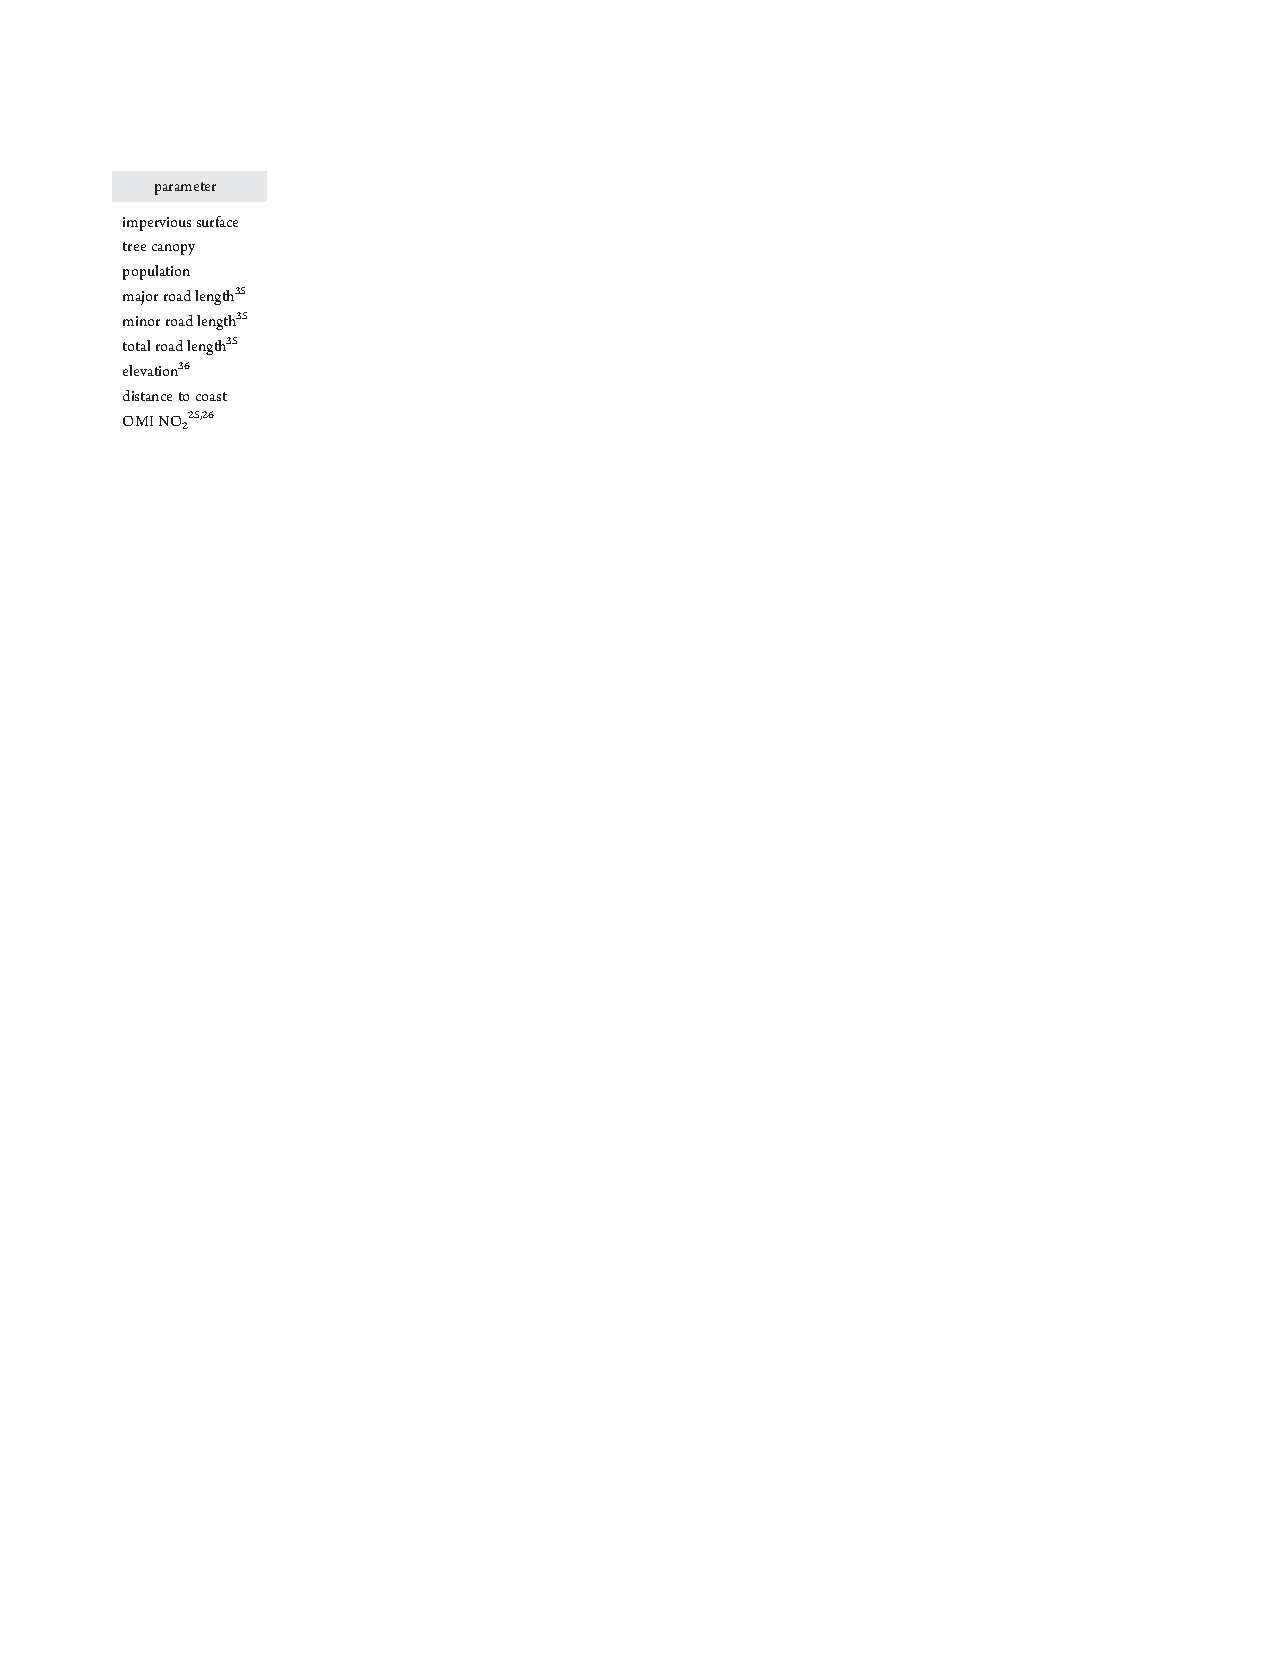
\includegraphics[height=0.5\textheight]{novotny_tab1_1}

\includegraphics[height=0.5\textheight]{novotny_tab1_2}
\hspace{10mm}
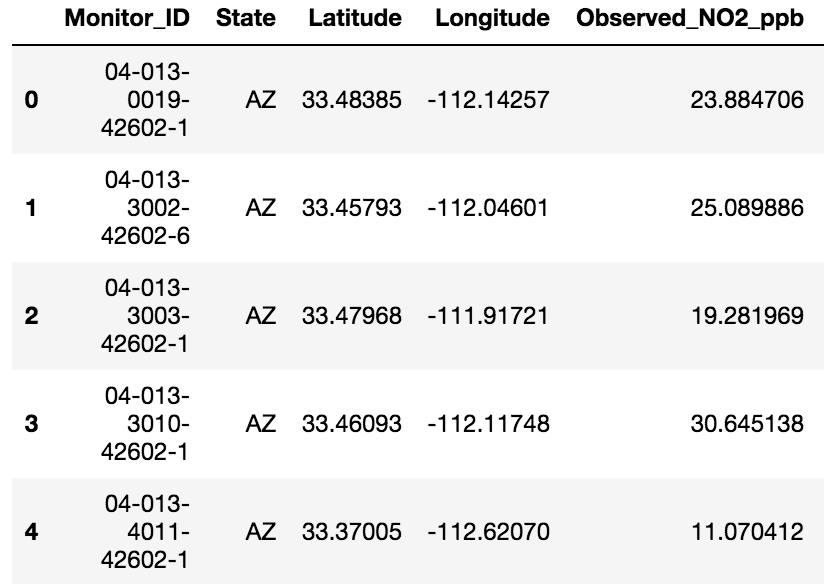
\includegraphics[scale=0.42]{novotny_DF}

\vspace{3mm}
The \textbf{State} variable could be treated as a qualitative predictor.

\vspace{3mm}

What about \textbf{Monitor\_ID}?  \pause Then each data point would have a unique intercept.  The model would overfit the data in the extreme.

\end{frame}

\begin{frame}{Can we do this?}



\vspace{5mm}

\begin{align*}
x \equiv \text{soup preference.}&\\
\text{Split pea} \rightarrow x &= 1\\
\text{Minestrone}  \rightarrow x &= 2\\
\text{Other}  \rightarrow x &= 3\\
\text{Don't like soup}  \rightarrow x &= 4
\end{align*}

\vspace{5mm}

Then fit some data, for example age of respondent, to $x$.
\pause

\vspace{5mm}

The problem with this mapping is that it forces the answers to be quantitative when they are not.

\vspace{3mm}\pause

We actually need need $n-1$ variables for $n$ mutually exclusive possibilities in a qualitative predictor.

\end{frame}

\begin{frame}{This is how you do it}

\begin{align*}
x_1 &=\begin{cases}
    1, & \text{Likes split pea}.\\
    0, & \text{otherwise}.
  \end{cases}\\
x_2 &=\begin{cases}
    1, & \text{Likes minestrone}.\\
    0, & \text{otherwise}.
  \end{cases} \\
x_3 &=\begin{cases}
    1, & \text{Doesn't like soup}.\\
    0, & \text{otherwise}.
  \end{cases}  
\end{align*}
 
  \textbf{Question:} What about the ``other'' category?  
  
  \pause
  
  \textbf{Answer: } The answers are mutually exclusive, so if $x_1, x_2, x_3$ are all zero, then the answer must be ``other''.

\end{frame}

\begin{frame}{Cooked-up example:  Predicting age}

\begin{align*}
\text{AGE}_i = \beta_0 + \beta_1 x_{1,i} + \beta_2 x_{2,i} + \beta_3 x_{3,i} + \beta_4 x_{4,i} + \epsilon_i
\end{align*}

where $x_{1}, x_2, x_3$ are defined on previous slide and $x_4$ is how spicy the respondent likes their food.

\vspace{5mm}

With these variables the qualitative predictors are just modifying the intercept.  
\begin{itemize}
\item When $x_1=x_2=x_3=0$ (i.e. the answer is ``other'') then the intercept is $\beta_0$.
\item Otherwise the intercept is $\beta_0+\beta_i$ where $i$ is the $x$ variable that is nonzero.
\end{itemize}

\end{frame}

\begin{frame}{Which equation belongs to which picture? (From ISLR)}

\vspace{3mm}
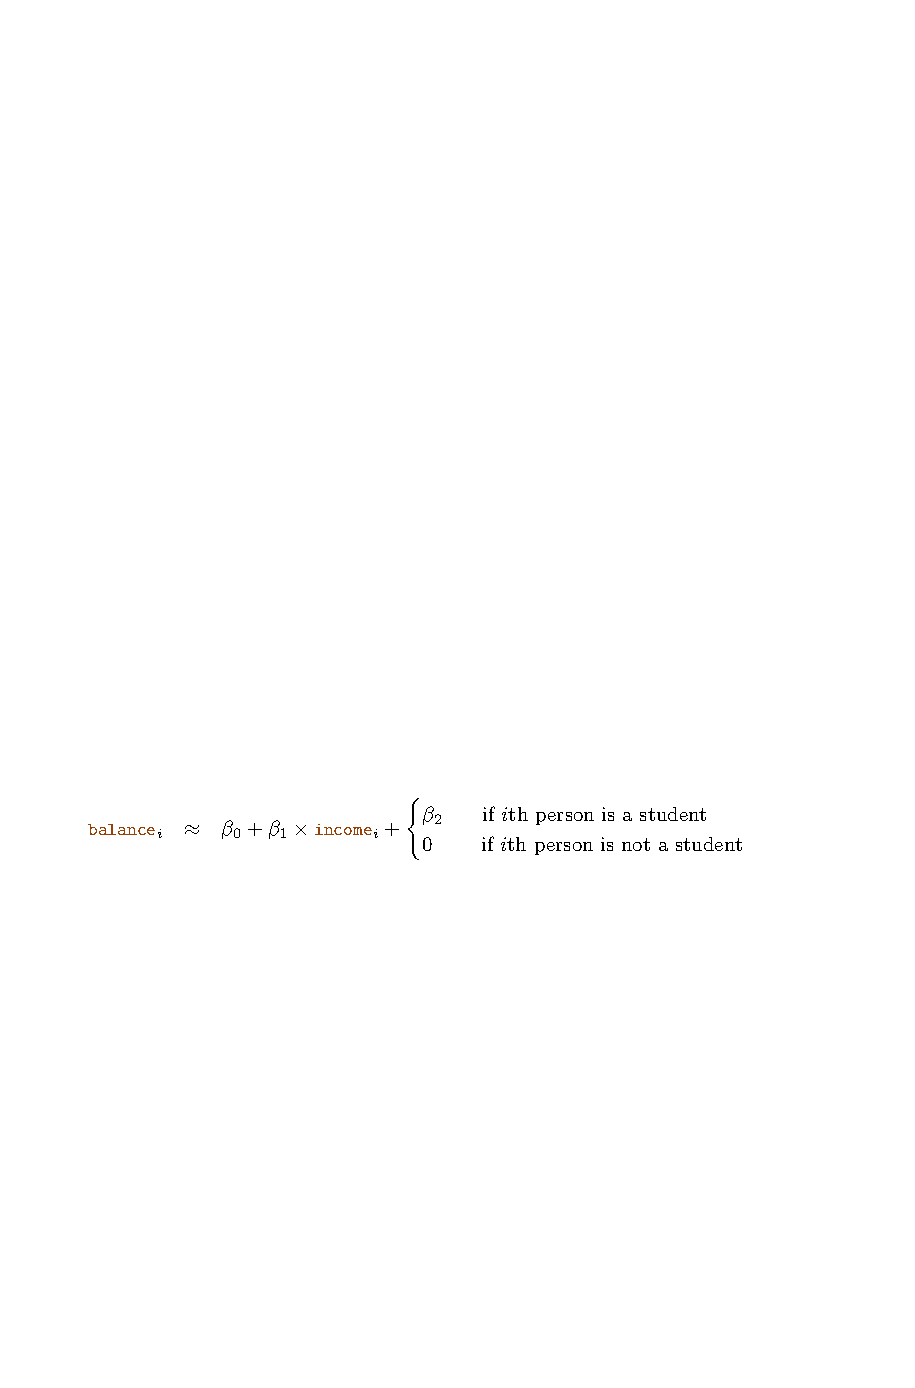
\includegraphics[width=0.8\textwidth]{CreditEqn1}

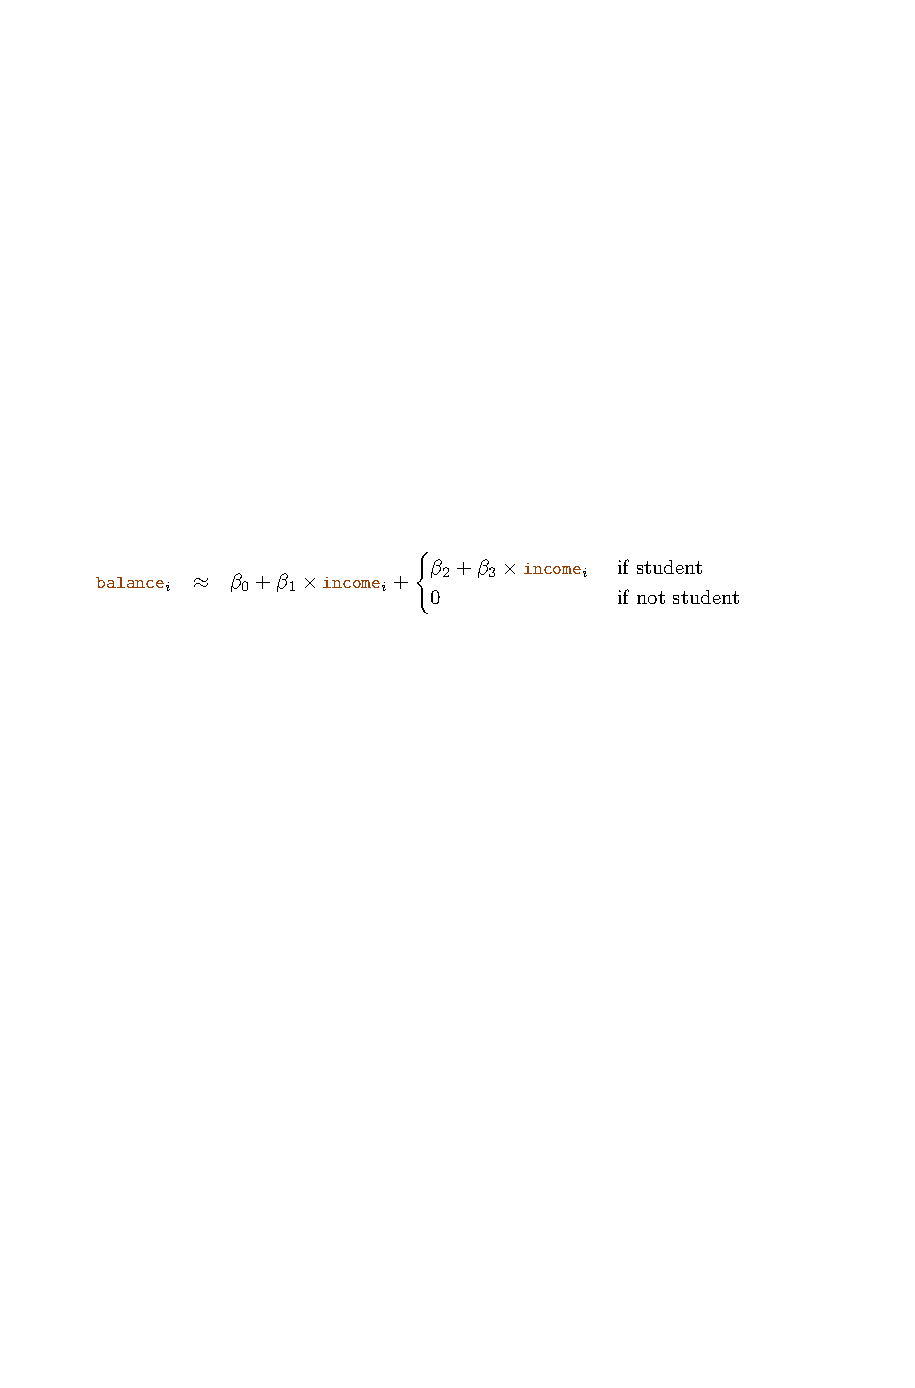
\includegraphics[width=0.8\textwidth]{CreditEqn2}

\begin{figure}
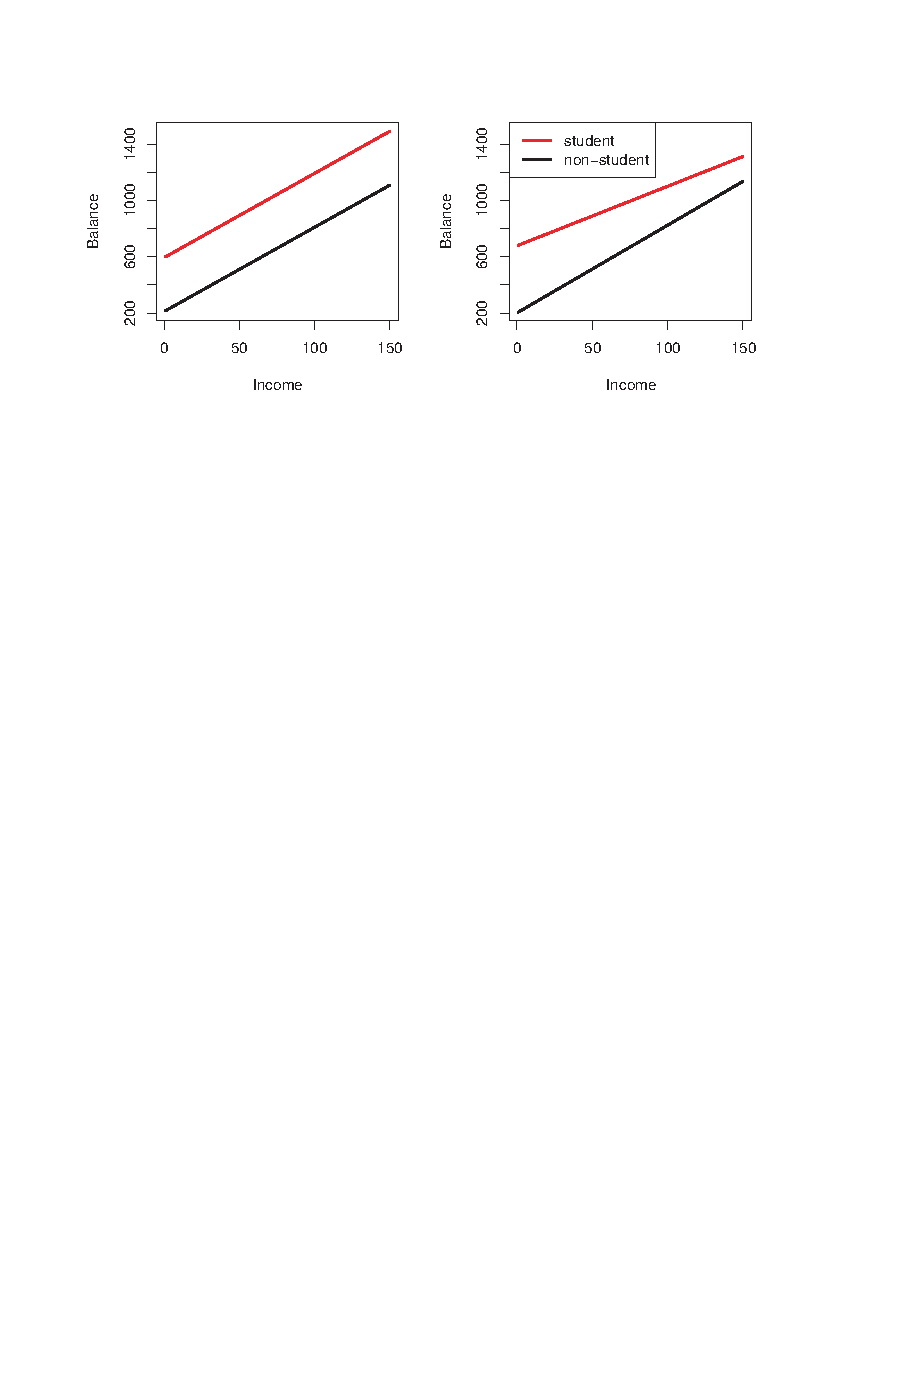
\includegraphics[width=0.8\textwidth]{CreditExample}
\caption*{}
\end{figure}
\end{frame}

\begin{frame}{Which equation belongs to which picture?}

\vspace{3mm}
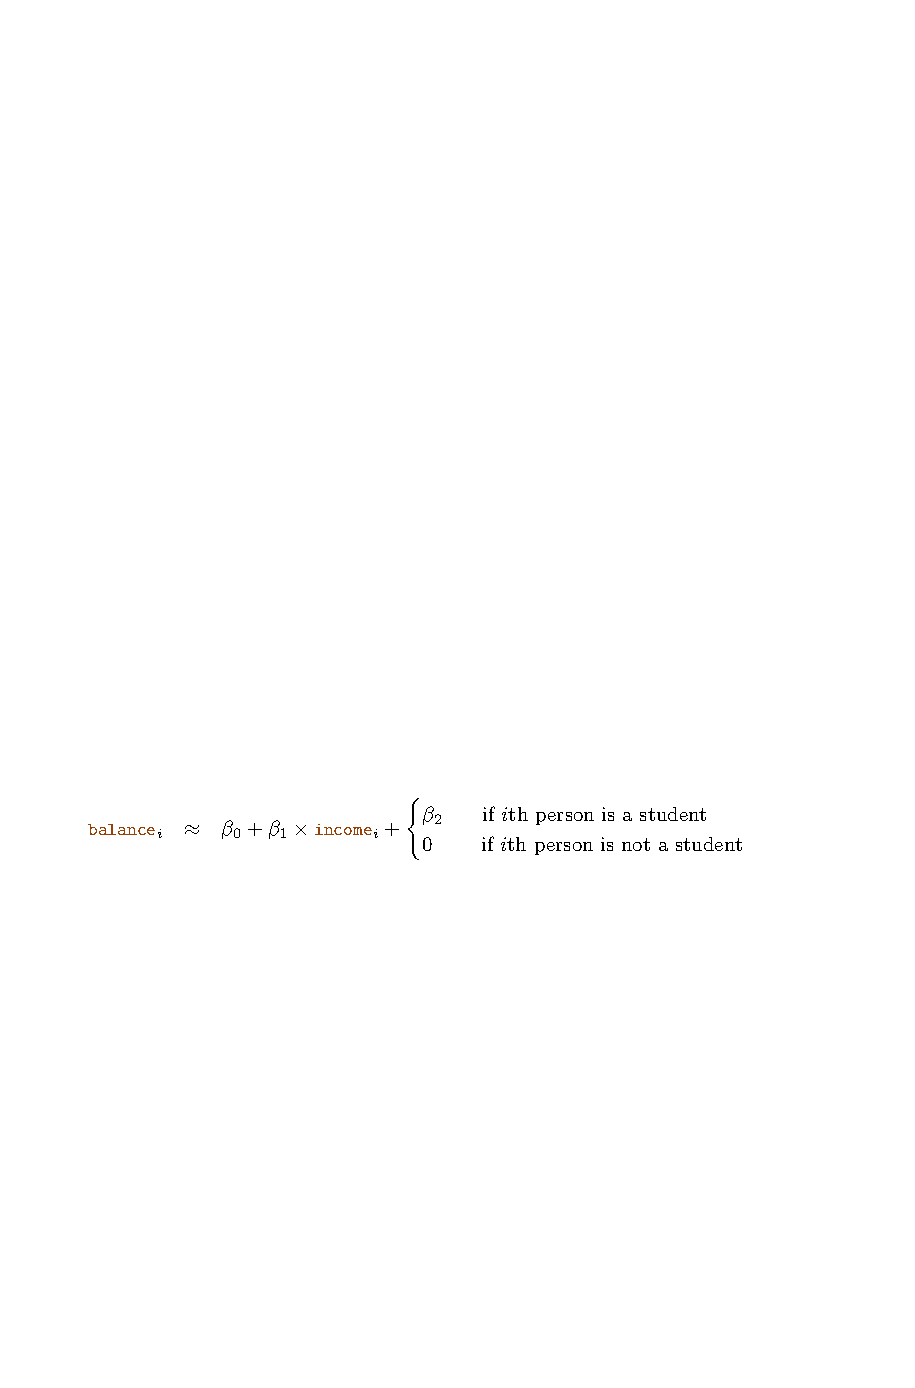
\includegraphics[width=0.8\textwidth]{CreditEqn1}

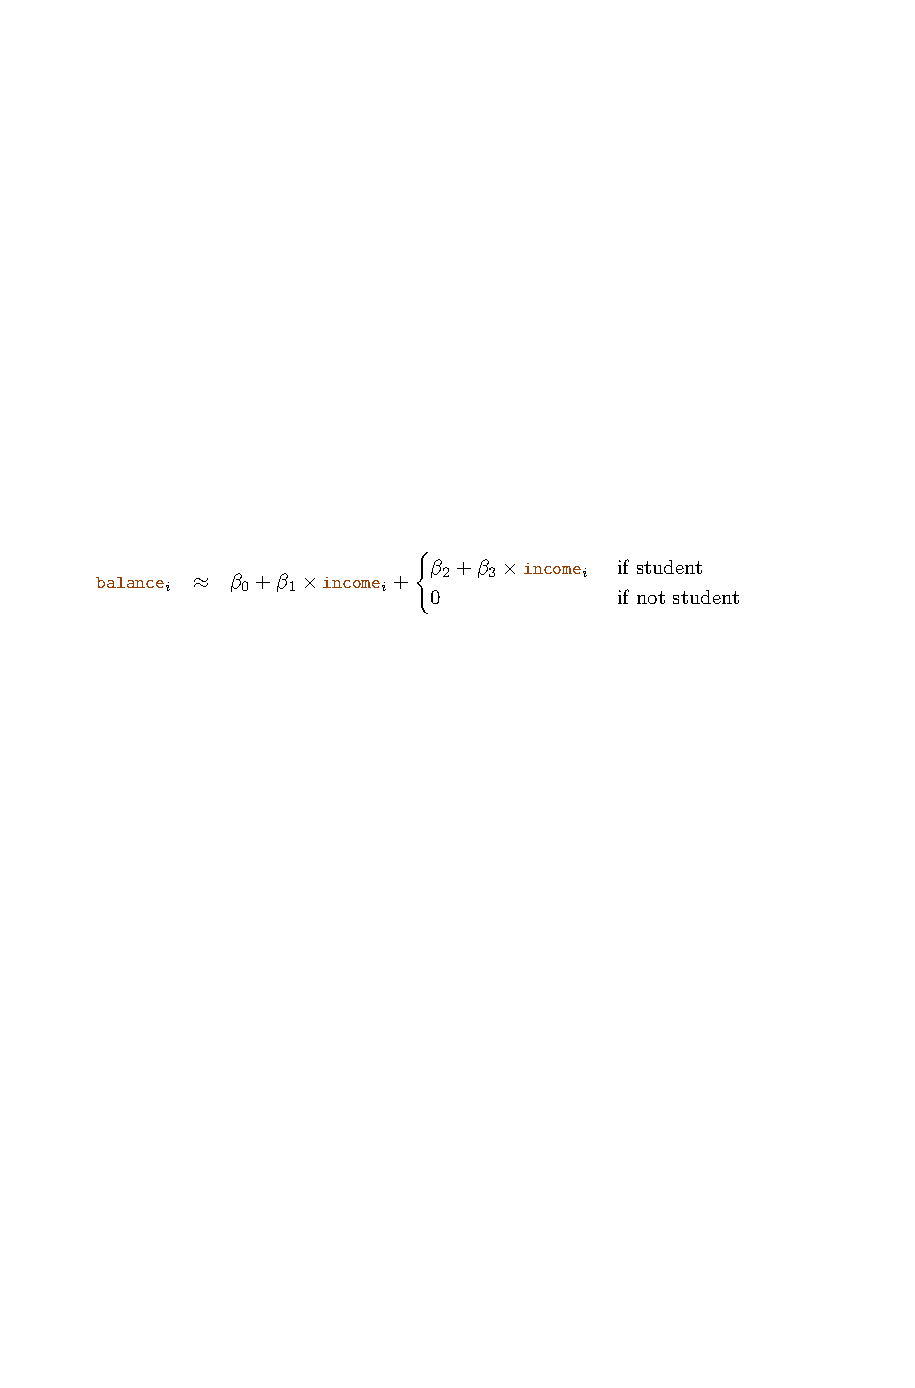
\includegraphics[width=0.8\textwidth]{CreditEqn2}


\vspace{3mm}

The first equation produces two lines with different intercepts $\rightarrow$ left figure.  

\vspace{3mm}

The second equation produces two lines with different intercepts \textit{and} slopes $\rightarrow$ right figure.  
\end{frame}

\begin{frame}{What if the relationship seems nonlinear?}

\begin{columns}
\column{0.65\textwidth}
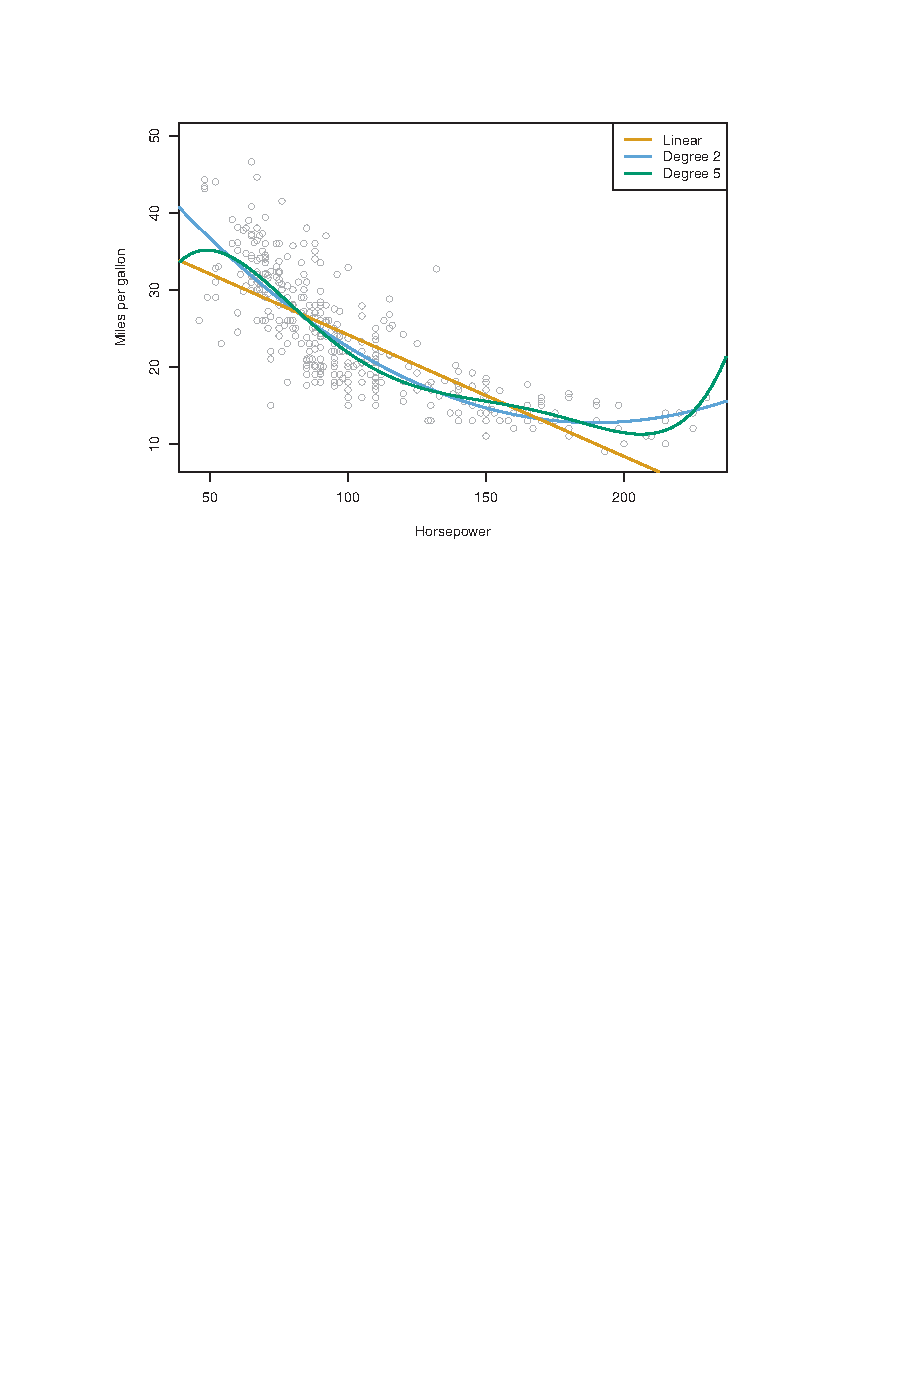
\includegraphics[width=\textwidth]{MPGvHorsepower}
\column{0.35\textwidth}
What's wrong with this statement:  We're doing \textit{linear regression}, so we can only capture \textit{linear relationships} between our data?

\vspace{5mm} \pause

\textbf{Answer:}  We can \textit{make} new nonlinear predictors to capture the relationship of interest.

\end{columns}
\end{frame}


\begin{frame}{Nonlinear predictors}

We can specify virtually any nonlinear model you can think of. For example:

\begin{align*}
\hat{y}_i = \beta_0 + \beta_1 x_i + \beta_2 x_i^2 + \beta_3 x_i^{\frac{1}{3}} + \beta_4 f(x_i)
\end{align*}

$f(x_i)$ can be any function you want!

\vspace{5mm}
Let's see how this might play out in the Novotny data. Check out the Lecture 11 Jupyter notebook.

\end{frame}

\begin{frame}{Potential problems}
  \begin{itemize}
    \item Non-linearity of the response-predictor relationships. 
    \item Correlation of error terms.
    \item Non-constant variance of error terms.
    \item Outliers.
    \item High-leverage points.
    \item Collinearity.  
  \end{itemize}
\end{frame}

\begin{frame}{Colinearity}

\begin{itemize}
\item Collineartity is the condition in which independent variables are strongly correlated with each other.  
\item It doesn't need to be that variable $x_j$ is correlated with variable $x_i$.  
\item For example, it could be that $2x_j+1.3x_k$ is correlated with $x_i$.
\item In other words, \textit{linear combinations} of variables could be correlated with each other.
\item \textbf{ Key problem: } results in inflated standard errors for coefficient estimates.  

\end{itemize}
\end{frame}

\begin{frame}{Colinearity -- example from ISLR. Plots show MSE contours}

\begin{figure}
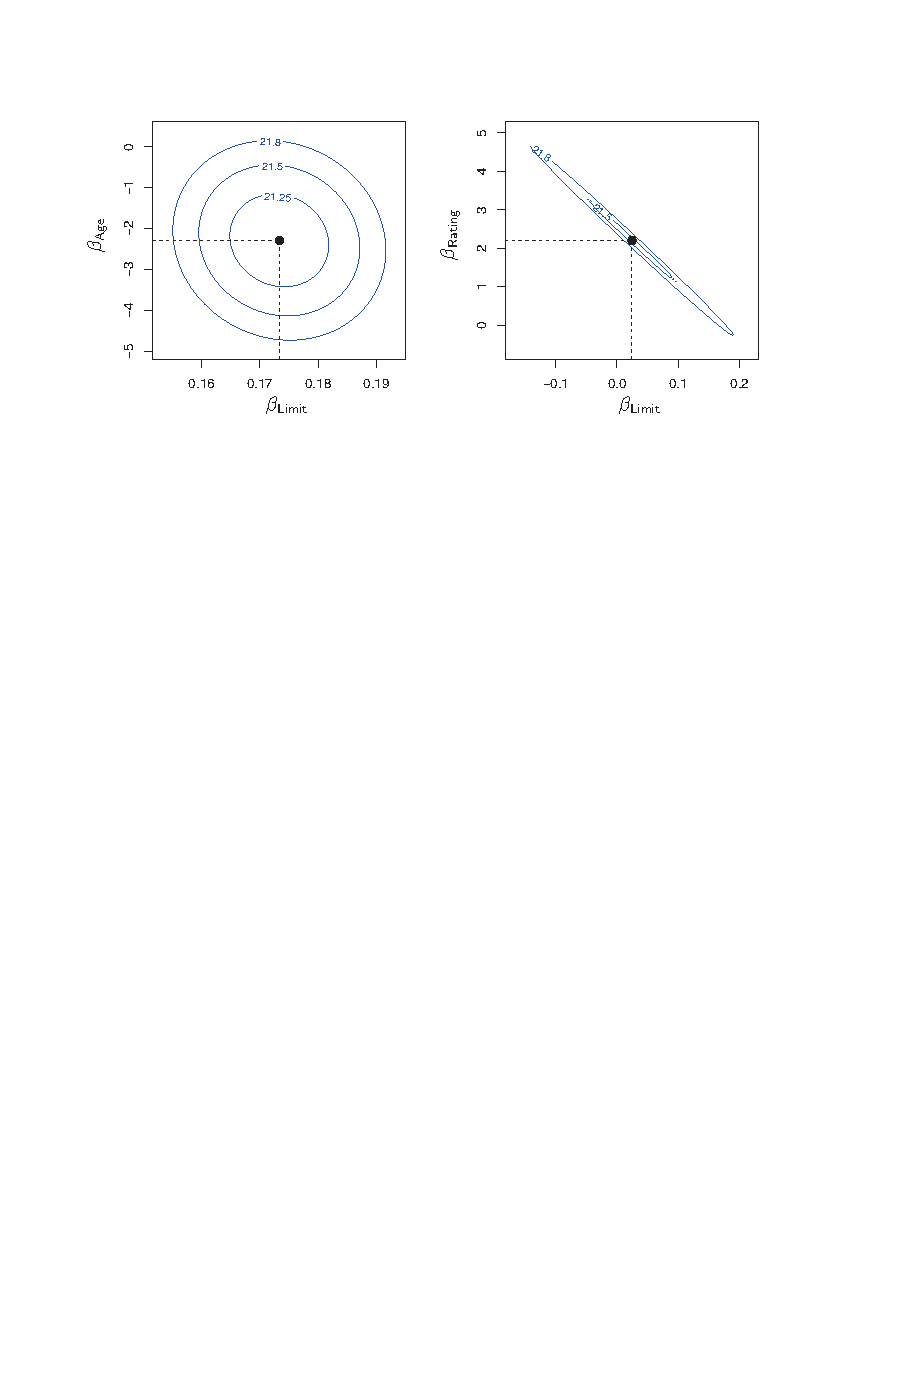
\includegraphics[height=0.7\textheight]{ISLR_fig3_15}
\caption*{}
\end{figure}

\vspace{-10mm}

Having such ``steep'' MSE contours makes the standard error, or variance, of the coefficients larger.  

\end{frame}


\begin{frame}{Variance inflation}

We can measure the extent to which collinearity seems to be impacting results by the VIF, or \textit{variance inflation factor}.

\begin{align*}
\text{VIF} &= \frac{\text{variance of $\hat{\beta}_j$ when fit with all other variables}}{\text{variance of $\hat{\beta}_j$ when it is the only independent variable}}\\
&\geq 1
\end{align*}

\vspace{5mm}

Novotny et al use VIF for feature selection.

\vspace{5mm}

\textbf{Question:} If we are focusing on prediction, should we care about evaluating VIF?


\end{frame}

\begin{frame}{K Nearest Neighbors regression}

This is a very simple non-parametric approach to regression.
\begin{itemize}
  \item Suppose we have a prediction point $x_0$.
  \item Identify the $K$ observations closest to $x_0$ 
  \begin{itemize}
    \item You'll need to choose a measure of distance -- Euclidean is common
  \end{itemize}
  \item Define $\mathcal{N}_0$ as the set of $K$ points
  \item KNN estimates $f(x_0)$ using the average of the output variables of the observations in $\mathcal{N}_0$.
\end{itemize}

\begin{align*}
  \hat{f}(x_0) = \frac{1}{K} \sum_{x_i \in \mathcal{N}_0} y_i
\end{align*}

\end{frame}





\end{document}


